\subsection{GeneNetwork}
GeneNetwork (\GN) is a large systems genetics platform that offers a lot of functionality to interested parties, mostly researchers~\cite{Williams:1994, Chesler:2004, Chesler:2005, Alberts:2010, Williams:2012, Mulligan:2017, Watson:2020}.
% \FIXME{Needs full list of GN publications}
\GN\ is funded by NIGMS as `GeneNetwork project to build a unified high performance FAIR  web service for systems genetics and precision medicine' (\textbf{R01 GM123489, 2017-2026}) and provides access to over 25 years of experimental data on mouse, rats and humans.
Functionality of this `toolbox system for genetics' can search genetic results, tissue correlation, browse (SNP), quantitative trait loci (QTL) mining and analysis. GN has a scriptable interface for querying its database, and an application programming interface (API) for linking we resources.
There is also a GeneWiki that allows crowd-sourced input from notes on genes and proteins to transcripts, with abundant search features.
GenomeGraph is yet another tool that allows viewing of global genetic modulation for many datasets for gene expression.
\GN\ has been used in over one thousand publications and is continuously updated~\cite{Watson:2020}.
One must note that \GN\ is not a simple tool, it is very involved and as new functionality is implemented, new instructional content must be made regularly.
\GN\ is an evolving platform with an active user base and consistently improving functionality.
\GN\ has been used for over one thousand publications, and as it is improved increased use is  expected by researchers involved in moving precision medicine forward\cite{Watson:2020}.

\subsection{BIG Project}
Precision medicine is an approach to the prevention and treatment of disease that takes into account differences in genes, environment and lifestyle to personalize recommendations by health care professionals. 
There have been dramatic medical success stories due to important health information obtained from genetic analysis: https://bit.ly/3yqketN.
However, the lack of clinical and genetic information available from socioeconomically disadvantaged populations threatens this goal and runs the risk of further increasing health disparities. 
In Tennessee, African Americans (especially in Memphis and Chattanooga) and rural populations, such as those in Appalachia (around Knoxville and Johnson City), are disproportionately impacted by chronic diseases and the associated costs of healthcare. 
Unfortunately, these populations have been severely underrepresented in both genetic studies and clinical drug trials, making precision medicine, with its promise of improvement in outcomes and long-term reduction in costs to the health care system, much more challenging for these groups. 

\subsection{From PageRank to GeneRank}
\subsubsection*{a. Rationale}

The point of gene-rank mechanism, at least the version most suitable to our aims, is to give researchers interesting sets of genes to study given a specific focus area.
For instance, when attempting to understand addiction the ability to both search over as many accessible sources as possible finding genes related to the topic and then being able to rank the `goodness' of the genes in a way that fits your `goodness' definition is a much desired tool for omics researchers.
Gunturkun\cite{Gunturkun:2022} et. al. have done the first part of this work at UTHSC with Pjotr Prins. 
They have developed \textit{Genecup}, a tool that mines for gene-keyword relationships from PubMed and the genome wide association studies catalogue\cite{Buniello:2019}.
Machine learning is used to disambiguate search topics, while the tool searches abstracts and finds genes with keywords together in the same sentence.
The tool builds an ontology to help support the searching of the databases, and upon fetching the information develops an interactive graph using the keywords, genes and articles it finds.
As the graph is interactive one can select nodes and investigate sentences from the abstracts that result from the user query.

Moving beyond this utility a gene-ranking mechnanism will be applied to the resultant genes listed with the returned results.
Why gene-ranking, because it can highlight genes and haplotypes -- a physical grouping of genomic variants that tend to be inherited together that typically reflects a unique combination of variants that reside near each other on a chromsome that can include a single or multiple genes \cite{NHGRI:Haplotype}.
We will quickly elaborate on some of the techniques before describing our methods.

\subsubsection*{b. Background}
Gene-ranking is not a new idea and has been looked into by several researchers over the years, as evidenced by many published works (e.g.~\cite{hero2004pareto, breitling2004, morrison2005, agarwal2009ranking, wu2012ranking, re2012fast, xiao2014novel, bourdakou2016discovering, deandres2016sensitivity, Botia:2021, Panigrahi:2021}).
In 2004 Breitling et al.\cite{breitling2004} determine the significance level of a gene by calculating a rank product (RP) on differential microarray gene expression over multiple samples.

When compared against significance of micro arrays (SAM) and fold change (FC) methods, RP outperforms SAM in every dimension and often agrees with FC.
While RP and the average-FC approach agree quite well on the datasets tested, it is found that RP is more robust against outliers, and performs well with small datasets with fewer replicates.

In 2005 this was followed by the GeneRank product by Morrison et al.\cite{morrison2005} which modifies \textit{Google's} PageRank \cite{langville2004deeper} algorithm for analyzing microarray experiments.
In an attempt to mirror the way webpages link to one another, hence driving their significance, GeneRank takes into account other gene connectivity data to determine a genes rank.
Some of the external data are functional annotations, protein interactions and previous experimental results.
By using and at times combining external data networks graphs can be built that show how genes are related to each other.
These network links are the functional equivalent of webpage links; therefore, the more nodes a gene is connected to helps determine its gene rank.
Following another aspect of the PageRank algorithm, GeneRank has its own version of random walk.
Random walk is related to the amount of time an individual would spend perusing a website when surfing the next.
With respect to gene ranking the random walk is the amount of time a biologist should spend looking at a gene whilst analysing the experimental results.
Fold changes (FC) are still important when using the GeneRank algorithm.
The study uses datasets whose networks are all created differently: one is built using gene ontology annotations of biological process, cellular component and molecular function, another is built using correlation coefficients between gene pairs and their expression changes intra experiment, and the last is a synthetic network that uses probabilities to connect genes in separate groups.
GeneRank is found to be able to create a list of important genes that are robust and do not rely only on expression change data.
It is concluded that this technique should not be used alone to get the measure of a genes importance and should be combined with expert knowledge and gene expression measurements.

In 2016 Zeng et al.\cite{zeng2016discovering} use PageRank\cite{langville2004deeper} for experiments without citing how it may have been modified for use with gene expression.
Differentially expressed genes (DEGs) are used to create the network necessary for PageRank calculations.
This work identifies databases from which relational information about genes is pulled, along with an analysis tool: the Gene expression omnibus (GEO) database (containing gene expression profiles), the Search Tool for the Retrieval of Interacting Genes (STRING) data (for predicting functional associations between proteins), and the Database for Annotation, Visualization and Integrated Discovery (\textit{DAVID}).
Like the work by GeneRank authors, gene ontologies are used with DEGs to create a network to find gene expressions related to psoriasis.
The top-ranked hub gene, estrogen receptor-1 (ESR1) was investigated thoroughly due to the output from the analysis, and multiple important observations were made.
One of the important observations is that ERS1 possesses anti-apoptic fuctions, and the pathway followed by ESR1 is the same as cancer pathways.
Zeng et al. use the PageRank algorithm to not only find expressive genes among many hundreds for a specific issue, but also find after investigation some relationships and behaviors of the gene that can lead to precision medicine.

More recent papers on gene rank go beyond looking to extend methods designed by Google and go into multivariate analysis using correlations \cite{Botia:2021} and multiple types of evolutionary computations \cite{Panigrahi:2021}, including particle swarm optimization (PSO), ant colony opmization (ACO), and differential evolution (DE).
Botia et.al. find univariate methods for gene ranking were lacking, in that they were ranking without paying attention to interactions between factors \cite{Botia:2021}. 
The author's methods use pairs of attributes in conjunction with a consistency metric for evaluating pairs together.
Evaluation of the techniques, the correlation-based feature selection (CFS) or \textit{Pairwise Correlation} and \textit{Pairwise Consistency}, was done with a gene expression dataset named \textit{gene expression cancer RNA-Seq} and \textit{GTEx RNA expression} that deal with brain tissue and brain age expression.
These techniques look at goodness of attributes and the consistency of the same to rank features.
Panigrahi et. al. write a review of methods used for gene-ranking in \cite{Panigrahi:2021}.
Many of the methods listed in their review include evolutionary computation and not just machine learning or correlative methodology.
Optimizers, particle swarm (PSO) and ant colony (ACO), are used in conjunction with other techniques to reduce dimensionality.
In these last few works, the methods are used to select genes for a classification task.
The classification task is not meant to find genes for investigation but to help predict an outcome, such is different from our stated interest while the techniques can still be useful in the work being pursued.

\subsubsection*{c. Methods}
One of the \GN\ innovative outcomes is to build a more powerful database system combining human and model organisms, where Mouse and rat will be combined in one data resource.
Data entry methods will undergo improvement by way of controlled vocabularies and ontologies to cover genotypes and phenotypes.
The improved database will use RDF+SPARQL which are technologies designed to make information on the web more interconnected and accessible.
Another added beauty of these technologies is that they are designed to speed up data access and querying, and most especially work optimally with AI tools.
Such linked data is explicitly encoded in a standardized machine-readable syntax with relations useful for machine learning exercises\cite{toh2019}.
Gene rank learner is a tool that will rely on data from multiple sources: pubmed, wikidata, \GN\, rat genome database (\href{http://rgd.mcw.edu}{RGD}), the gene expression omnibus (GEO)~\cite{NCBIGeo}, the search tool for the retrieval of interacting genes (STRING~\cite{STRING}), the database for annotation visualization and integrated discovery (DAVID~\cite{DAVID}), a new human gene database collected from volunteers~\cite{henderson2020}, and more.
One of the major aspects of this software will be a data management service that pulls ontologies, schema and other functional data information so that querying data from different sources is done transparently as if there is one large data source. 
In essence, creating a sort of data lake with bridges to different sources and an adaptive interface that supports quick addition of more data sources.
The initial algorithm implemented will be gene rank product used by Zeng et.al. in \cite{zeng2016discovering}, along with a function to count fold changes.
Correlation and consistency algorithms will be implemented next, as they take gene expression information into account, improving upon the significance of micro arrays (SAM) methods that would focus on gene expression yet were outperformed by gene rank product in the past.
An ant colony optimizer (ACO)~\cite{ACO:2009} will be implemented to traverse the large graph that will be created from the accumulation of data from the various sources.
ACO looks for optimal solutions using graph traversal; hence, we must define what we think to be a possible optimal set of interesting genes based off of a genes many characteristics.
Each of these algorithms will be compared against one another by being made available to the \GN\ community.
Those who use the gene rank learner will be encouraged to provide feedback.
Before being released to the \GN\ community we will provide multiple definitions of interesting genes, and compare the efficacy of the results from each technique.
This ensemble of algorithms will be implemented in the Julia programming language, some of the packages that will be used are \hyperlink{https://www.juliapackages.com/p/antcolony}{a package for using ant colony optimization -- antcolony}, \hyperlink{https://juliapackages.com/p/evolutionary}{a package for evolutionary computations -- evolutionary}, \hyperlink{https://juliapackages.com/p/mxnet}{a package to run ML algorithms with GPU optimization -- MXNet}, and the \hyperlink{https://alan-turing-institute.github.io/MLJ.jl/dev/}{a general ML framework -- MLJ}.


\subsection{Causal Inference Investigations}
In thinking through a causal diagram for diabetes, because its complications lead to so many other serious issues in underrepresented communities, we need to look at causes that mediate and ones that are confounders.
A list of causes that can be evaluated: damage to the pancreas, obesity, specific medicines, high cholesterol, age, family history and certain hormonal conditions/imbalances.
The following list are things that are not easily evaluated or known: genetic predisposition, genetic mutation, lifestyle, gestational complications, and chance.
In the causal diagram `genetic mutation', healthcare access, and lifestyle all connect to the outcome diabetes through mediators.
Mediators are like symptoms to a problem, while explaining a known subset of a cause a mediator does not encompass the full probability of a cause that effects a specific outcome.
Even with mediators the furthest causes from the outcome do not all have a direct line to the outcome in our diagram in order to make the diagram less confusing and complicated.
A much more simple diagram could have been created with three nodes with the two cause nodes representing the group of observable causes and the group of unobservable causes both having a direct connection to the diabetes outcome.
However, this oversimplification does not help with showing the minimal complexity for the onset of diabetes.
For instance, `genetic mutation' is unobservable, as is `genetic predisposition' while both being confounders.
Also when looking at the several mediators from `genetic mutation' I am using `genetic predisposition' as a catch all past the mutation, since there are three other mediators based off of that single cause.
These causes are Confounders because especially as combined with `family history' and `lifestyle' can be interchanged and swapped and reach the diabetes outcome, with high probability while also being able to `prevent' diabetes if any one is not attributable to an individual.
Then there are causes like `age' and `specific medicines' that can directly bring the onset of diabetes while not logically being able to be a lone catalyst for the same.
However, the diagram must be based off of our current knowledge and refined as we learn more, just like a machine learning model.

\captionsetup{font={scriptsize,sc,up,singlespacing}}
%\begin{figure}[h] % Figure at bottom of the page ([b] argument, could be "t" for top or "h" for here)
%	\centering
%	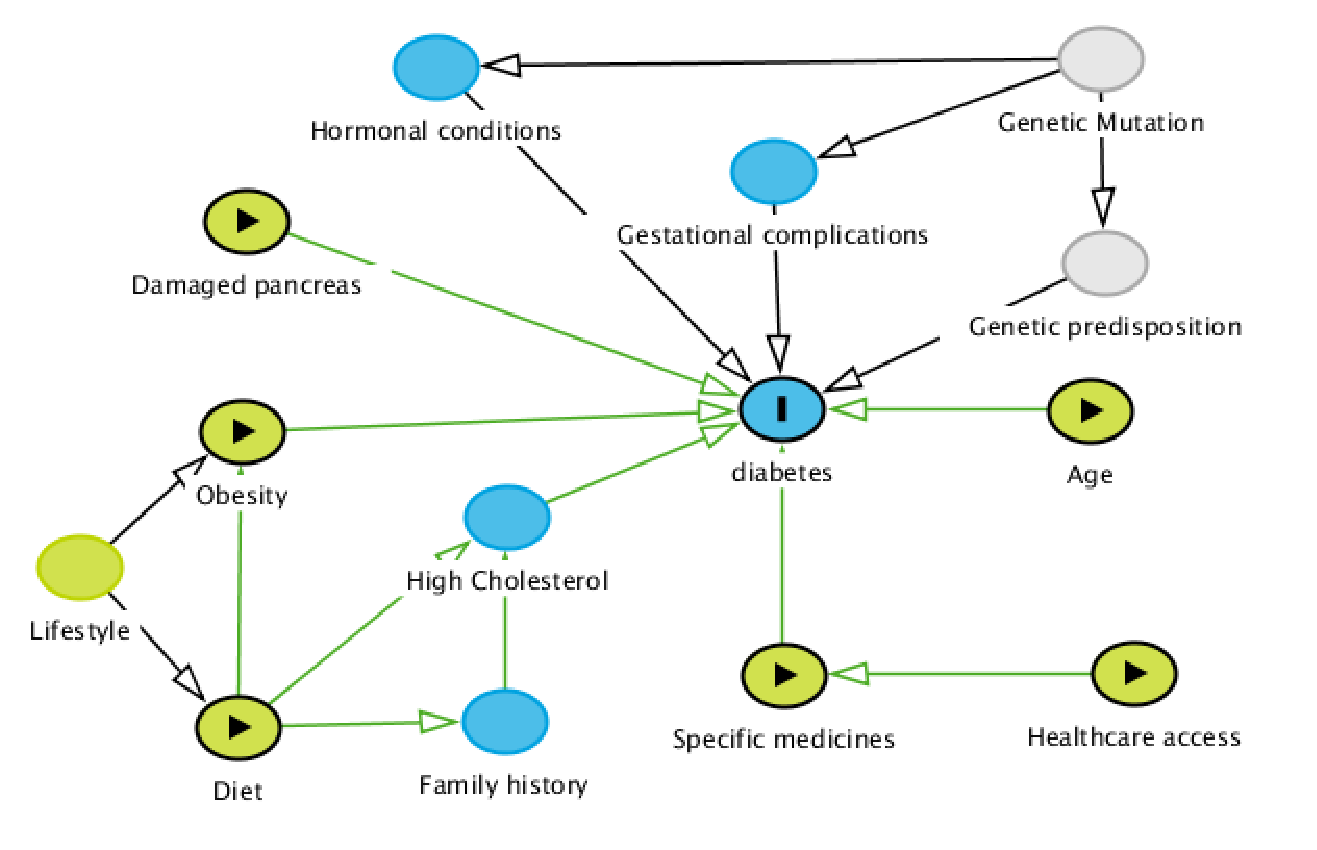
\includegraphics[width=.8\textwidth]{diabetes-causalmodel}
%       \label{fig:diabetes-cm}
%\end{figure}

\begin{figure*}[ht]\centering % Using \begin{figure*} makes the figure take up the entire width of the page
	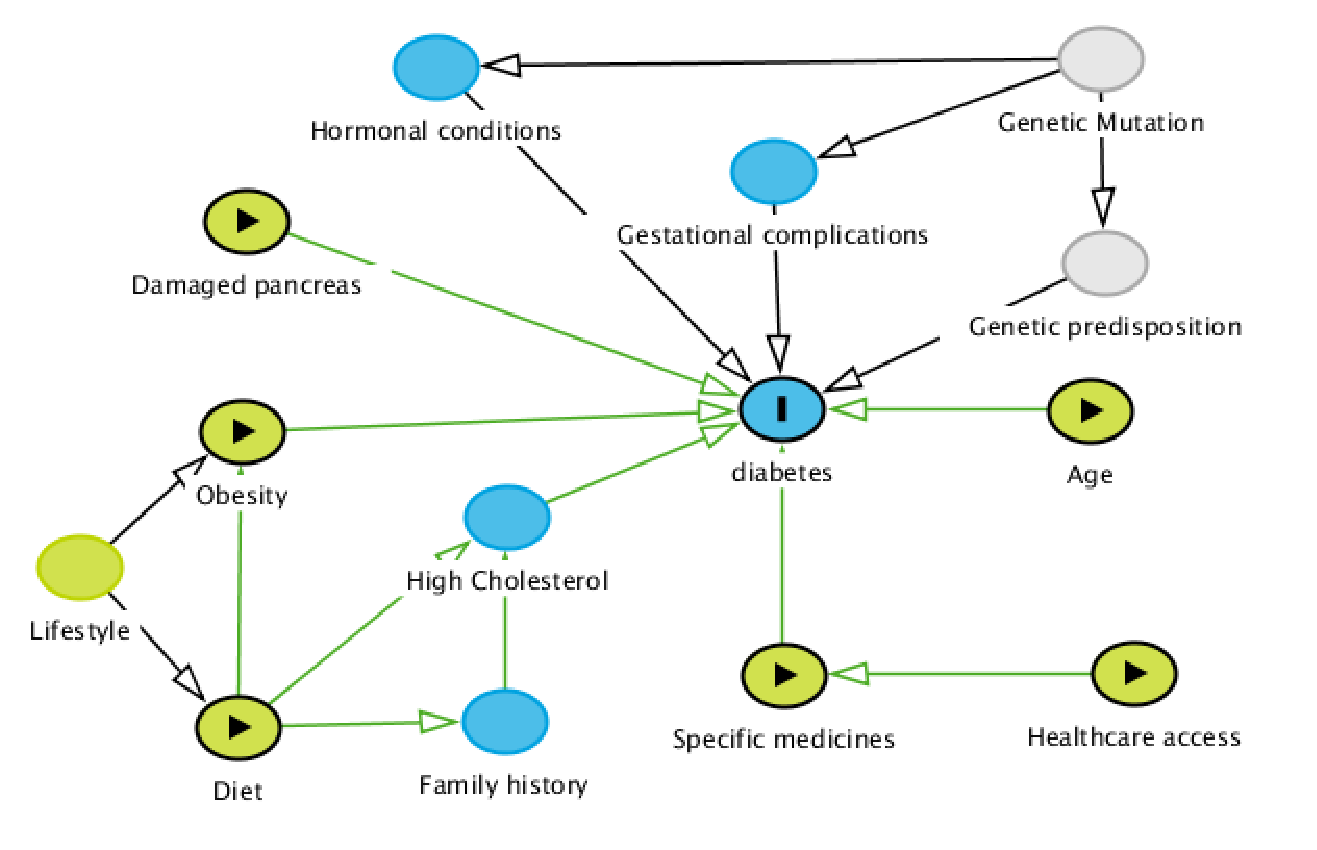
\includegraphics[width=\linewidth]{diabetes-causalmodel.eps}
	\caption{ \textbf{Example of a graphical causal model for diabetes that can be used for probablistic and causal reasoning:}
diabetes is a complex disease where simple GWAS deliver significant SNP hits that do not necessarily lead to new treatments because of confounding factors, including environment and genetic variants that differ between people. This is especially relevant for individuals belonging to minorities.
Some of Shelby Solomon's postdoc research will explore AI-type inferencing mechanisms using Judea Pearl's graphical models for probabilistic and causal reasoning: starting from the existing Bayesian network webserver (BNW) logic that is already in GeneNetwork Shelby Solomon will, in the long-term, add AI-type inferencing mechanisms to see if we can improve scale and logic and expose these tools through the \GN\ user interface.
The goal is to get answers to causal questions about specific health issues, including asthma, sickle cell disease, and epilepsy in the BIG cohort. In \GN\ we will also target gout, diabetes, high blood pressure, and heart disease by exploring over 25 years of mouse and rat studies.
        }
	\label{fig:diabetes-cm}
\end{figure*}